
\begin{itemize}
	\item Ciarlet: the finite element method for elliptical problems (1987/2002)\\
	\item Brenner, Scott: the mathmatical theory of finite element method (2002)\\
	\item Schmidt, Siebert: design of adaptive finite element software
\end{itemize}



\section{Beispiele}

\begin{align*}
	\Delta u &= f \quad  in\  \Omega\\
		   u &= 0 \quad auf\ \partial\Omega
\end{align*}

$\rightarrow$ \underline{finite Differenzen}\enter
\enter
z.B. $\Omega = (0,1) \times (0,1)$ mit der Notation
\begin{align*}
	 u&= u(x,y)				 &   u_{ij}&\ \text{approximiert}\ u(x_i,y_j)\\
	(x_i, y_j) &\in \Omega, \quad i,j = 1,\dots,N&  h&= x_{i+1} - x_i = y_{i+1}-y_i
\end{align*}

-Taylorentwicklung
\begin{align*}
	u(x_{i+1},y_j) &= 	u(x_{i},y_j) + 	h\partial_x u(x_{i},y_j) + \frac{1}{2}h^2 \partial_{xx}	u(x_i,y_j) + O(h^3)\\
	u(x_{i-1},y_j) &= 	u(x_{i},y_j) - 	h\partial_x u(x_{i},y_j) + \frac{1}{2}h^2 \partial_{xx}	u(x_i,y_j) + O(h^3)\\
\end{align*}

$\implies$
\begin{align*}
	\partial_{xx} u(x_i,y_j) &= \frac{1}{h^2}\left(	u(x_{i+1},y_j) - 2u(x_i,y_j) + 	u(x_{i-1},y_j) \right) + O(h)\\
	\partial_{yy} u(x_i,y_j) &= \frac{1}{h^2}\left(	u(x_i,y_{j+1}) - 2u(x_i,y_j) + 	u(x_i,y_{j-1}) \right) + O(h)
\end{align*}

$\implies$
\begin{equation*}
	\Delta u(x_i,y_j) = \frac{1}{h^2} \left( u_{i+1 j} + u_{i-1 j} + u_{i j+1} + u_{i j-1} - 4u_{i j} \right)
\end{equation*}

$\implies$
\begin{align*}
	 u_{i+1 j} + u_{i-1 j} + u_{i j+1} + u_{i j-1} - 4u_{i j} &= f_{i j}h^2 & & (x_i,y_j) \in \Omega\\
	 u_{i j} &= 0 & & (x_i,y_j) \in \partial\Omega 
\end{align*}

Benenne die $u_{ij}$ in $u_k$ um, mit $k = iN+j$. Bezeichne nun $U_k = u_{ij}$ und $F_k = f_{ij} $.

$\implies$
\begin{equation*}
	AU = F 
\end{equation*}
mit 
\begin{align*}
	A = \frac{1}{h^2}
	\begin{pmatrix}
	A_0       & I        & 0		&\dots  & 0     \\
	I		  & A_0 	 & I 		&\ddots & \vdots\\
	0		  & I        & \ddots 	&		& 0     \\
	\vdots    & \ddots   & 		  	& A_0	&	I   \\
	0		  & \dots 	 & 0  		& I 	& A_0   \\
	\end{pmatrix}, 
	\quad
	A_0 = 
	\begin{pmatrix}
	-4    		& 1      & 		  & \textbf{0}  \\
	1	  		& -4 	 & \ddots & 			\\
		  		& \ddots & \ddots &	1   \\
	\textbf{0}	& 	     & 1 	  & -4   \\
	\end{pmatrix}
\end{align*}

%% maybe Vor- und Nachteile

$\rightarrow$ \underline{finite Elemente}\enter
\enter
\begin{align*}
\Delta u &= f \quad  \text{in}\  \Omega\\
u &= 0 \quad \text{auf}\ \partial\Omega
\end{align*}

\begin{equation*}
	\int_\Omega \Delta u v \diff x = \int_\Omega fv \diff x \text { f\"ur } v\in C^1(\overline{\Omega}), \; v=0 \text{ auf } \partial \Omega
\end{equation*}

\begin{align*}
	\int_\Omega \text{div}( \nabla u) v \diff x
	 &= \int_\Omega \text{div}( v \nabla u ) \diff x -	\int_\Omega \nabla u \cdot \nabla v \diff x \\
	&=  \underbrace{\int_{\partial\Omega}  v \nabla u  \cdot \vartheta \diff x}_{=0\text{ s. Def. v}} -	\int_\Omega \nabla u \cdot \nabla v \diff x \\
	&=  \int_\Omega fv \diff x
\end{align*}

Dies gilt für $u \in X$ s.d. $\forall v\in X$ f\"ur einen passenden Funktionenraum $X$.
Diese Form wird schwache Formulierung oder Variationsformulierung.
\enter
Gesucht wird eine Approximation $u_h$ in endlich dimensionalen Raum $X_h$ s.d. $X_h \to X$ f\"ur $h \to 0$.\enter
$u_h$ erf\"ullt f\"ur alle $v\in X_h$ die Gleichung
\begin{equation*}
	-	\int_\Omega \nabla u_h \cdot \nabla v_h \diff x = \int_\Omega fv_h \diff x.
\end{equation*}

Sei $\varphi_1,\dots, \varphi_n$ eine Basis von $X_h$, dann gilt:
\begin{equation*}
	u_h = \displaystyle\sum_{i=1}^N u_i\varphi_i 
\end{equation*}
und mit $v=\varphi_j$ folgt 
\begin{equation*}
	- \displaystyle\sum_{i=1}^N u_i \int_\Omega \nabla \varphi_i \cdot \nabla \varphi_j \diff x = \int_\Omega f\varphi_j \diff x \qquad j=1,\dots,N
\end{equation*}
mit 
\begin{align*}
	A_{ij} = \int_\Omega \nabla \varphi_i \cdot \nabla \varphi_j \diff x, \quad \quad F_j = \int_\Omega f \varphi_j \diff x
\end{align*}
$\implies$
\begin{align*}
	- \displaystyle\sum_{i=1}^N A_{ij}u_i &= F_{ij}\\
	AU &=F
\end{align*} 

W\"ahle nun $\varphi_j$ mit kleinem Tr\"ager.\enter
\begin{equation*}
	\text{spt}(\varphi_j) = \overline{\left\{  x \in \Omega: \varphi_j(x) \neq 0 \}\right}
\end{equation*}

%  Obige schreibweise gefällt mir nicht

Definiere $\varphi_j(b_i) = F_{ij}$ und $\varphi_j$ linear in allen Teilabschnitten $\tau \in T$, wobei $T$ eine Triangulierung ist und 
\begin{equation*}
	\overline{\Omega} = \displaystyle\cup_{\tau\in T}\ \tau
\end{equation*}
gilt.

\begin{figure}[!h]
	\centering
	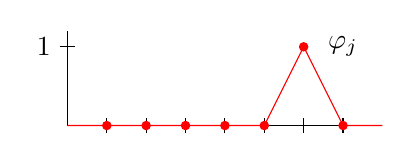
\begin{tikzpicture}[scale=1]

	
	%\fill[black!20!white] (2.15,0) -- ++(0,0.35) -- ++(0.65,0.26) -- ++(0,-0.61) -- cycle;
	%\draw (2.15,0) 
	\draw (0,0) -- ++(0,1.2);
	\draw (0,0) -- ++(4,0);

	\draw[red] (0,0) -- ++(2.5,0) -- ++(0.5,1) -- ++(0.5,-1) -- ++(0.5,0);
	%\filldraw (2.15,0.35) circle (0.4pt);
	
	\draw (-0.1,1) -- ++(0.2,0);
	
	\draw (0.5,-0.1) -- ++(0,0.2);
	\draw (1  ,-0.1) -- ++(0,0.2);
	\draw (1.5,-0.1) -- ++(0,0.2);
	\draw (2  ,-0.1) -- ++(0,0.2);
	\draw (2.5,-0.1) -- ++(0,0.2);
	\draw (3  ,-0.1) -- ++(0,0.2);
	\draw (3.5,-0.1) -- ++(0,0.2);
	
	
	\filldraw[red] (0.5,0) circle (1.5pt);
	\filldraw[red] (1  ,0) circle (1.5pt);
	\filldraw[red] (1.5,0) circle (1.5pt);
	\filldraw[red] (2  ,0) circle (1.5pt);
	\filldraw[red] (2.5,0) circle (1.5pt);
	\filldraw[red] (3  ,1) circle (1.5pt);
	\filldraw[red] (3.5,0) circle (1.5pt);
	
	
	\node at (-0.3,1) {1};
	\node at (3.5,1) {$\varphi_j$};
	%\node at (2.8,-0.1) {b};
	%\node at (2.15,0.53) {f(a)};
	%\node at (2.77,0.71) {f(b)};
	
	\end{tikzpicture}
\end{figure}